%%
%% This is file `sample-sigconf.tex',
%% generated with the docstrip utility.
%%
%% The original source files were:
%%
%% samples.dtx  (with options: `sigconf')
%%
%% IMPORTANT NOTICE:
%%
%% For the copyright see the source file.
%%
%% Any modified versions of this file must be renamed
%% with new filenames distinct from sample-sigconf.tex.
%%
%% For distribution of the original source see the terms
%% for copying and modification in the file samples.dtx.
%%
%% This generated file may be distributed as long as the
%% original source files, as listed above, are part of the
%% same distribution. (The sources need not necessarily be
%% in the same archive or directory.)
%%
%%
%% Commands for TeXCount
%TC:macro \cite [option:text,text]
%TC:macro \citep [option:text,text]
%TC:macro \citet [option:text,text]
%TC:envir table 0 1
%TC:envir table* 0 1
%TC:envir tabular [ignore] word
%TC:envir displaymath 0 word
%TC:envir math 0 word
%TC:envir comment 0 0
%%
%%
%% The first command in your LaTeX source must be the \documentclass command.
\documentclass[runningheads]{llncs}
%\documentclass[sigconf]{acmart}

% If you use the hyperref package, please uncomment the following line
% to display URLs in blue roman font according to Springer's eBook style:
% \renewcommand\UrlFont{\color{blue}\rmfamily}

\usepackage{pgfplotstable}

%\setlength {\marginparwidth }{2cm} % not part of original template
\usepackage[colorinlistoftodos]{todonotes}
%\usepackage{tabularx}
\usepackage{multirow}
\usepackage{pgfplots}
\usepackage{enumitem}
% Make citations clickable
\usepackage[hidelinks]{hyperref}
\pgfplotsset{compat=1.17}
\usetikzlibrary{calc}


%% These commands are for a PROCEEDINGS abstract or paper.
%\acmConference[K-Cap '21]{K-Cap '21: The Eleventh International Conference on Knowledge Capture}{December 02--03, 2021}{Virtual Conference}


%%
%% Submission ID.
%% Use this when submitting an article to a sponsored event. You'll
%% receive a unique submission ID from the organizers
%% of the event, and this ID should be used as the parameter to this command.
%%\acmSubmissionID{123-A56-BU3}

%%
%% The majority of ACM publications use numbered citations and
%% references.  The command \citestyle{authoryear} switches to the
%% "author year" style.
%%
%% If you are preparing content for an event
%% sponsored by ACM SIGGRAPH, you must use the "author year" style of
%% citations and references.
%% Uncommenting
%% the next command will enable that style.
%%\citestyle{acmauthoryear}

%%
%% end of the preamble, start of the body of the document source.
\begin{document}

%%
%% The "title" command has an optional parameter,
%% allowing the author to define a "short title" to be used in page headers.
\title{OntoFlow: A user-friendly Ontology Development Workflow}
%\titlerunning{OntoFlow}

\author{
	Gordian Dziwis\orcidID{0000-0002-9592-418X} \and
	Lisa Wenige\orcidID{0000-0002-3707-3452} \and
	Lars-Peter Meyer\orcidID{0000-0001-5260-5181} \and
	Kirill Bulert\orcidID{0000-0002-1459-3754} \and
	Michael Martin\orcidID{0000-0003-0762-8688}}
% "authorrunning" needed to get rid of page header "Authors Suppressed Due to Excessive Length"
\authorrunning{G. Dziwis et al.}
\institute{Institute for Applied Informatics, Goerdelerring 9, 04109 Leipzig, Germany \email{\{dziwis,wenige,lpmeyer,bulert,martin\}@infai.org}}

%% example author and institute info from template
%\author{First Author\inst{1}\orcidID{0000-1111-2222-3333} \and
%Second Author\inst{2,3}\orcidID{1111-2222-3333-4444} \and
%Third Author\inst{3}\orcidID{2222--3333-4444-5555}}
%%
%\authorrunning{F. Author et al.}
%% First names are abbreviated in the running head.
%% If there are more than two authors, 'et al.' is used.
%
%\institute{Princeton University, Princeton NJ 08544, USA \and
%Springer Heidelberg, Tiergartenstr. 17, 69121 Heidelberg, Germany
%\email{lncs@springer.com}\\
%\url{http://www.springer.com/gp/computer-science/lncs} \and
%ABC Institute, Rupert-Karls-University Heidelberg, Heidelberg, Germany\\
%\email{\{abc,lncs\}@uni-heidelberg.de}}

%%
%% This command processes the author and affiliation and title
%% information and builds the first part of the formatted document.
\maketitle

%%
%% The abstract is a short summary of the work to be presented in the
%% article.
\begin{abstract}
	For many years, the development of widely applicable and high quality ontologies has been an ongoing research topic. Among the various challenges, the lack of integrated development environments for non-technical domain experts has been one of the most pressing research issues. But while the participation of domain experts is vital for the applicability of ontologies, there are hardly any software tools available that facilitate their active engagement. We present a solution that addresses this research gap by automating the ontology development process with the help of a workflow engine. We define a pipeline that facilitates ontology implementation, serialization, documentation and testing within the scope of a seamless automatic routine than can be easily set up by the ontology engineer and triggered by a non-technical domain expert. Thus, the processing pipeline takes care of most of the operations that usually have to be carried out by an ontology or software engineer. We demonstrate the applicability of the approach by developing an ontology with OntoFlow and validating its functioning with a large-scale ontology dataset from Linked Open Vocabularies (LOV).
\end{abstract}

%%
%% Keywords. The author(s) should pick words that accurately describe
%% the work being presented. Separate the keywords with commas.
\keywords{Ontology \and Workflow \and Integrated Development Environment \and Quality Assurance}

\section{Introduction}
With the proliferation of knowledge graphs, ontology development has become a central part of data integration activities. Due to the increasing efforts around FAIR data and research data infrastructures worldwide \cite{fair}, collaborative and decentralized processes around ontology development are on the rise. However, available software tools fall short of the multi-layered requirements of ontology development which comprise labour-intensive tasks such as ontology modeling, serialization, validation and documentation. Moreover, these tasks often have to be carried out collaboratively and in a decentralized manner as several (often geographically dispersed) groups of people are involved in the ontology development process thus making it a multi-stakeholder endeavor \cite{sure}. In addition to that, many of the tools available are difficult to handle for domain experts without IT or Semantic Web background \cite{tudorache}. While these experts have an extraordinarily high level of expertise in their field (e.g., in life sciences, physics or cultural heritage) they might not be as familiar with the methods and tools commonly applied in software and knowledge graph engineering. This situation is exacerbated by the fact that there exists no standard tool stack for ontology development in the Semantic Web community. Although some tools, such as Protégé \cite{protege}, are considerably widespread, they only cover partial aspects of the engineering process such as ontology modeling or editing and cannot be used in the sense of a fully-fledged integrated development environment (IDE). On top of that, many software tools for RDF file processing can either only be used as a command-line utility and/or provide limited usability in terms of a graphical user interface (GUI). However, virtualisation and continuous integration (CI) techniques from software engineering provide novel opportunities for ontology development \cite{fowler} and can also help to ease participation of domain experts.\\
With OntoFlow we propose a solution that bundles several necessary operations of ontology engineering in a single automated workflow by adopting best practices from CI pipelines \cite{humble}. Thus, we are able to integrate ontology modeling, serialization, testing and documentation in a unified process which makes time-consuming, repetitive and error-prone manual work mostly superfluous.
The paper is structured as follows: Section~\ref{sec:related} provides an overview of current practices of workflow automation for data collections and highlights existing gaps in software-based support for ontology development processes. Section~\ref{sec:ontoflow} introduces requirements, architecture and implementation-specific details of the OntoFlow approach. Section~\ref{sec:eval} presents results of the evaluation of the OntoFlow approach, while the final Section~\ref{sec:final} summarizes the most important findings and proposes directions for future work.
\section{Related Work}\label{sec:related}
Continuous development and integration strategies have become an indispensable part of modern software engineering.
They largely consist of clean-up operations, compilation of executables, application of automated tests, and the deployment of the finished application, including generation of appropriate documentation if necessary. Part of these processes is the constant checking of any updates/new versions as well as the triggering of troubleshooting activities if problems occur~\cite{fowler}.
This ensures that software solutions are always up-to-date, that applications meet predefined quality standards and rely on stable software artifacts. Likewise, in the wake of ever-growing data volumes and increased relevance of data-driven applications, effective mechanisms to control the quality-assured publication of data products are required for IT operations. Processes that follow CI principles are equally needed for efficient production of data artifacts. The knowledge graph community has been one of the first to adopt DevOps best practices for datasets since it heavily relies on high quality data schemas and reproducible workflows for data conversion, integration and fusion. In this line of research, several authors have proposed automated data pipelines that take care of data transformation, apply quality assurance operations and automatic procedures for data publication and effective description of data artifacts~\cite{cirulli,klimek,kucera,meissner,rojas,roman,stadler,dataid}. CI mechanisms for data collections involve operations such as crawling, linking, or data transformation. These processes are usually executed automatically and are not interrupted by user interactions and manual intervention. If people work with software tools in this context, they are mostly data scientists or software engineers.\\
This modus operandi differs from the determining factors in ontology development. The creation of an ontology usually involves several experts with diverse backgrounds and different levels of technical expertise. Therefore, an effective ontology development environment/pipeline has to foster collaboration as well as provide a graphical editor in order to effectively support development processes. By this means, even domain experts with no IT expertise can actively take part in the creation of ontologies.\\
Ontology editors such as Protégé~\cite{protege}, OntoSeer~\cite{ontoseer}, Vocol~\cite{halilaj} or WebVOWL~\cite{lohmann} are already established software tools for ontology development and visualisation. Additionally, the Semantic Application Design Language offers an English-like language for semantic modeling.\footnote{\url{https://github.com/SemanticApplicationDesignLanguage/sadl}} Other applications in this area focus more on aspects of collaborative and version-based storage of ontologies so that changes can be managed decentrally and tracked over time. Software tools, such as Ontoology~\cite{alobaid} or the QuitStore~\cite{arndt} provide solutions for these kinds of requirements.\\
Tools, such as Oops! focus more on the aspect of quality assurance~\cite{poveda} while general purpose RDF data testing tools, such as RDFUnit~\cite{rdfunit} or pySHACL~\cite{sommer} can be equally applied for ontology testing. Just as important as quality assurance of ontologies is documentation for end users. Software applications that automatically generate ontology documentations are WIDOCO~\cite{widoco}, LODE~\cite{lode} or pyLODE\footnote{\url{https://github.com/RDFLib/pyLODE}}. They create a HTML representation from ontologies in standard RDF serialization formats. WIDOCO even goes beyond the purely automatic creation of ontology documentation by enabling metadata enrichment or ontology testing. However, it does not provide an easy-to-use interface for domain experts. Moreover, it is a Java-based monolithic software which makes modifications and extensions with tools from other technology stacks (e.g., Python-based software applications) difficult.\\
The ROBOT framework offers many operations needed for ontology manipulation in the development process, but lacks workflow capabilities. The framework's documentation refers to the rather technical oriented \textit{Make}\footnote{\url{https://www.gnu.org/software/make/}} tool for more complex needs.\\
Although some existing software applications already support collaborative ontology development processes and also automate them in parts, there is a lack of approaches as to how these processes can be linked in the sense of a CI pipeline while at the same time ensuring that laymen can actively participate in ontology engineering through making changes and triggering updates~\cite{mungall}.
\section{Ontology Development Workflow}\label{sec:ontoflow}
\subsection{Requirements}

\begin{table*}[hbt]
	\caption{Requirements for OntoFlow}
	\renewcommand{\arraystretch}{1.3}
	%\begin{tabular}{|p{0.25\textwidth}|p{0.75\textwidth}|}
	\begin{tabular}{p{0.4\textwidth} p{0.6\textwidth}}
		%\begin{tabulary}{\textwidth}{ |L|L| }
		\hline
		\multicolumn{2}{c}{\textbf{RQ1 ODP Automation}}                                                                                  \\
		\hline\hline
		RQ1.1 Ontology Serialization  & Ontology artifacts can be automatically serialized in common RDF formats                         \\

		RQ1.2 Ontology Validation     & Automatic testing of ontology artifacts is integrated                                            \\

		RQ1.3 Ontology Postprocessing & Integrating automatic postprocessing operations, such as version control or diff detection       \\

		RQ1.4 Ontology  Documentation & Automatic creation of a HTML ontology documentation                                              \\

		RQ1.5 Ontology Publication    & Automatic deployment of ontology artifacts (serialization and HTML documentation) to a server    \\
		\hline
		\multicolumn{2}{c}{\textbf{RQ2 High (Re-)Usability}}                                                                             \\
		\hline
		\hline
		RQ2.1 GUI support             & Support of ontology modelling through a graphical user interface                                 \\

		RQ2.2 Easy Execution          & Domain experts (with little to no IT background) should be able to trigger ontology workflows    \\

		RQ2.3 Fast Execution          & It should be possible to quickly generate an ontology, validate it and create its documentations \\

		RQ2.4 Easy Modification       & Ontology developers should be able to modify them easily to suit their individual requirements   \\
		\hline
	\end{tabular}\label{tab:req}
\end{table*}

The goal of OntoFlow is the best possible optimization and automation of ontology development processes which typically currently involve a great number of labor-intensive tasks, such as modeling, serialization, updating, testing and documentation. Due to the fact that such development processes are carried out by several stakeholders, the workflow environment should foster a collaborative and decentralized way of working.\\
Since the development of ontologies often involves domain experts who have only limited expertise in the field of software and data engineering, OntoFlow should provide a GUI for editing the ontology while automating the most common tasks (e.g., bash scripting and \textit{Git} interaction) in the background. Due to the limited IT experience of some of the involved stakeholders, it is also vital that workflows can be triggered without in-depth technical understanding of software development or semantic technologies. Reducing the amount of necessary skills for the domain expert is critical, because generally ontology development is a one time job for them. A reusable ontology workflow setup directed at domain experts helps avoiding costs for learning the involved technologies and setting up a development and hosting infrastructure (e.g., running a web server for publishing the ontology and documentation) which - apart from working time - can incur further costs for licences and hardware. Because there is no standard established methodology for ontology development and it happens in diverse environments, OntoFlow must be flexible and facilitate easy modifications to accommodate for different needs. Table \ref{tab:req} gives an overview of the requirements detailed in the above sections.

\subsection{Workflow Structure}
Figure~\ref{fig:workflow} gives an overview of the workflow. Data inputs for the workflow are generated by the ontology developer. He/she provides ontology diagrams, OWL files and validation shapes. An ontology diagram is a visual representation of an ontology. The OWL files define ontologies with the Web Ontology Language (OWL) and are serialized as an RDF file. The schema is tested with SHACL shapes to ensure that it satisfies certain conditions. A set of validation shapes, which test the compliance to best practices for ontology development are supplied by OntoFlow.

The first process is the transformation of the ontology diagrams to OWL files and merging those with (potentially existent) other OWL files provided by the user. The resulting ontology is the input for the following processing steps carried out in parallel:
A HTML documentation is generated, describing the ontology's metadata, classes and properties. The ontology is serialized into multiple RDF formats. During validation, the ontology is tested against some previously defined SHACL shapes. If needed, OntoFlow can be adapted so that the publication of the ontology fails whenever certain SHACL constraints are violated.
OntoFlow picks up the `owl:priorVersion` property and detects semantic differences to the previous version. This gives an overview which classes changed in the current version compared to the previous one. The serializations, documentation and validation reports as well as the semantic differences compose the Ontology Artifact Package.
%\begin{figure}[hb]
\begin{figure}[htb]
	\centering
	%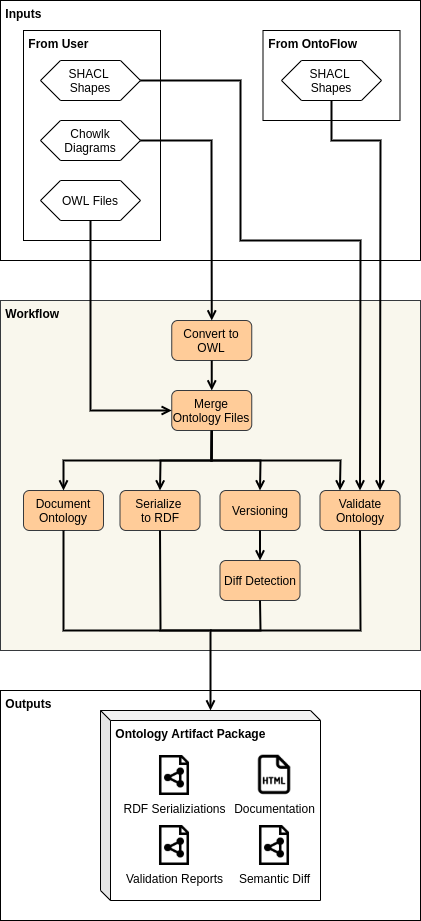
\includegraphics[scale = 0.555]{workflow.png}
	%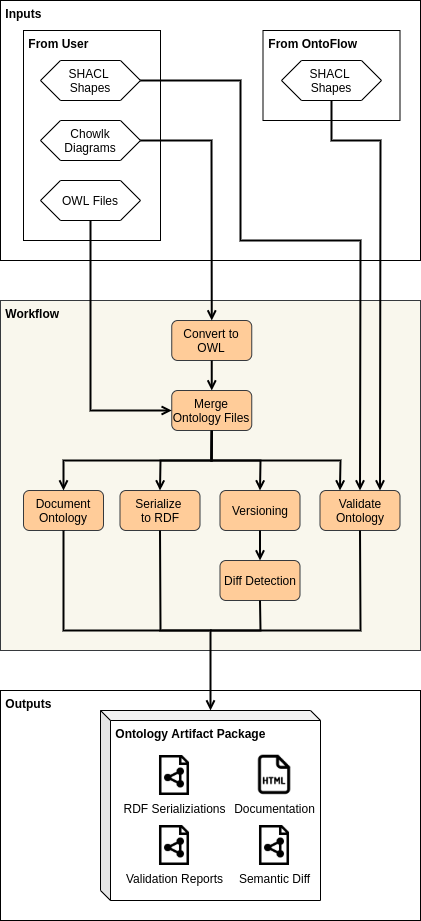
\includegraphics[width=.45\textwidth] {workflow.png} %preserves space
	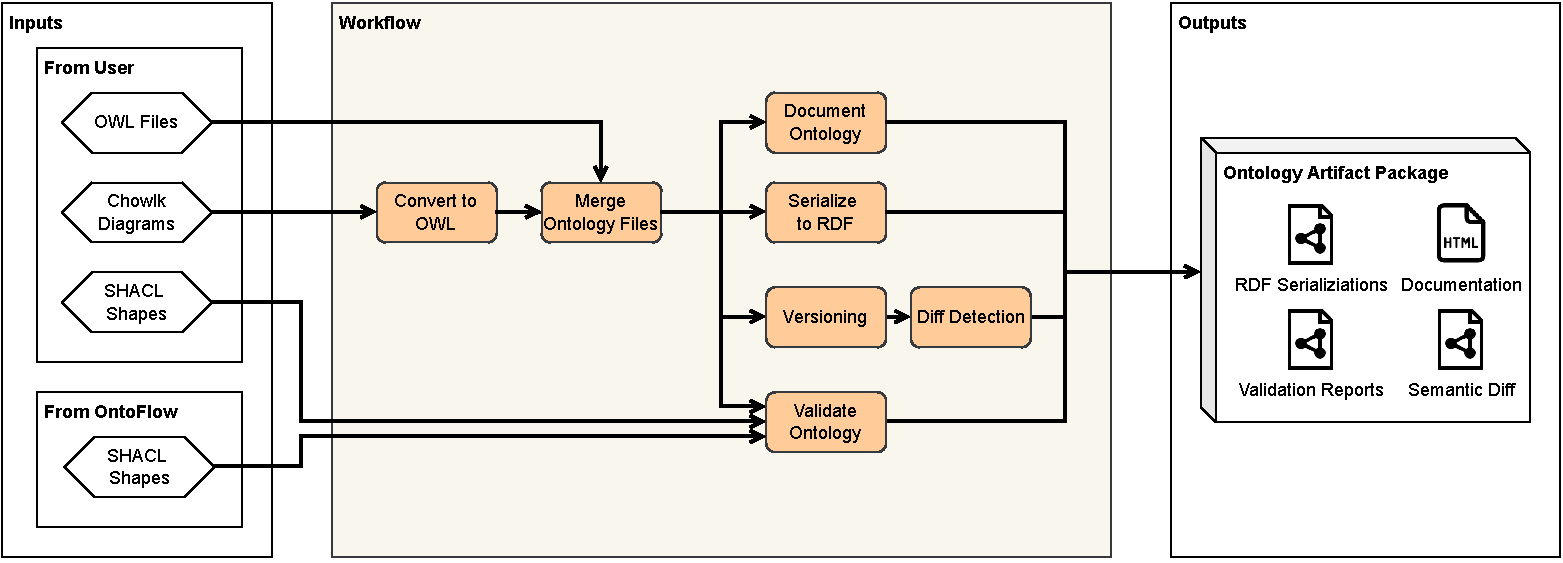
\includegraphics[width=\textwidth] {workflow_landscape.pdf}
	\caption{OntoFlow Workflow}\label{fig:workflow}
\end{figure}

\subsection{Implementation and Architecture}

The architectural model of OntoFlow is a pipeline consisting of processes where each operation takes inputs, transforms them and outputs the results. Process inputs and outputs are interconnected. Operations are carried out by different application programs with a command-line interface. All applications are containerised and the container images are defined by a configuration file. A workflow engine manages container life cycles, executes the applications and pipes the inputs and outputs between the processes. The pipeline operations with their executing containers and commands as well as inputs and outputs are defined in a workflow file. Each application container is based on an image for which a configuration file exists. There is a container for OntoFlow itself which has all the necessary dependencies for running the workflow engine. The images are hosted in a container registry. A continuous integration script builds the images and pushes them to the registry. Image as well as ontology files are managed inside \textit{Git} repositories to enable version control.

OntoFlow provides a continuous integration script, which is triggered whenever a change in the ontology repository occurs. When executed, the OntoFlow container is started with the mounted ontology repository. Inside the container, the engine initializes the workflow with the files from the ontology repository and OntoFlow's validation shapes as inputs. Each process step is then executed in its defined application container. The final outputs are deployed to their target environment.

The pipeline was implemented as a Nextflow \cite{Tommaso} workflow and Docker was chosen as the container engine. For each tool used in a process step, a Docker image was chosen or created, if it not already existed. The following list describes the software tools used in OntoFlow:

\begin{itemize}
	\item Chowlk Converter and draw.io\footnote{\url{https://github.com/oeg-upm/Chowlk}}: Converts the ontology diagrams to OWL files. Chowlk\cite{ChavezFeria} provides a library of OWL diagram elements for draw.io\footnote{\url{https://app.diagrams.net/}} which is an open source diagram software.
	\item pySHACL: Validates the ontology against SHACL shapes.
	\item Bubastis\footnote{\url{https://github.com/EBISPOT/bubastis}}: Creates a semantic \textit{diff} in comparison to an older ontology version.
	\item Jena Riot\footnote{\url{https://jena.apache.org/documentation/io/}}: Serialises and merges RDF files.
	\item sparql-integrate\footnote{\url{https://github.com/SmartDataAnalytics/RdfProcessingToolkit}}: Extracts and manipulates data in RDF files.
	\item pyLODE: Creates the ontology documentation in HTML.
\end{itemize}
OntoFlow can be run on any Linux system with Java and Docker installed which facilitates easy modifications and extensions. OntoFlow is integrated into the GitLab ecosystem thus boosting the options for automation. GitLab's container registry hosts the tool images and its continuous integration infrastructure is utilized for running OntoFlow. The Ontology Artifact Package is hosted as a GitLab page. With the schema files managed in a GitLab repository, it is possible to edit the ontology collaboratively, because draw.io can use a GitLab repository as its storage backend. This also works when multiple persons are editing the same diagram. This provides the option for collaborative editing without the user needing to explicitly interact with \textit{Git}. Chowlk diagrams are draw.io diagrams of an ontology or parts of an ontology. They are defined with elements from the Chowlk Ontology Visual Notation library, exported to an XML File. A line-wise diff comes for free through the usage of a \textit{Git} repository. For documentation purposes, the semantic \textit{diff} provided by Bubastis\cite{malone} gives a more useful overview over the changes between ontology versions. Bubastis analyzes and reports on the five major types of ontology changes.
%\begin{figure}[t]
\begin{figure}[htbp]
	\centering
	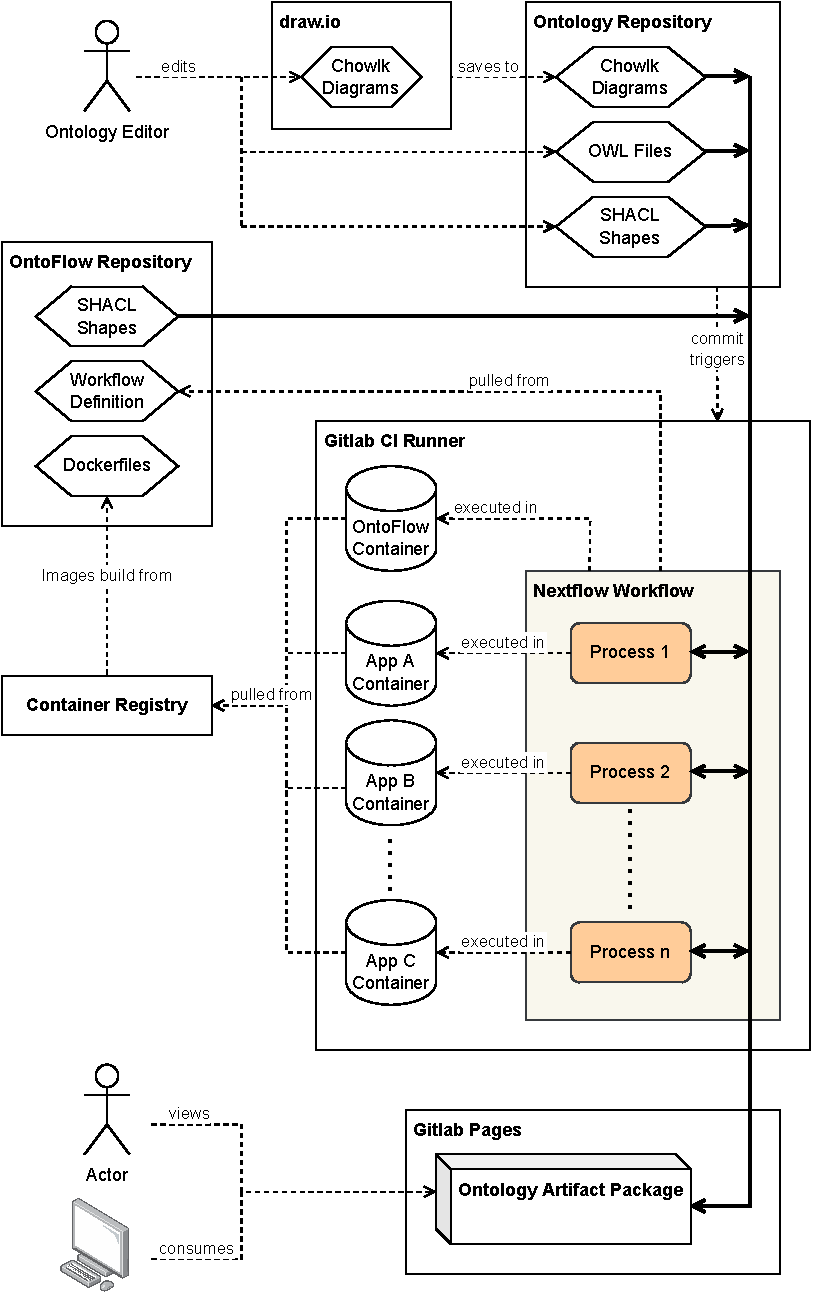
\includegraphics[width=.75\textwidth]{architecture.pdf}
	\caption{OntoFlow Architecture}
	\label{fig:architecture}
\end{figure}
Before an ontology \textit{diff} can be created, the serialized file and location of the previous ontology version has to be determined. To achieve this we run a custom SPARQL query against the input RDF file with sparql-integrate and output the URI locating the prior ontology version.

We curated a set of tools which fulfill our functional requirements, packaged each in a Docker container, wired them together with Nextflow and integrated the resulting workflow with the GitLab ecosystem.
The OntoFlow code and documentation are available on GitLab, so that anyone interested can use the software and see how the tool works.\footnote{\url{https://gitlab.com/infai/ontoflow}}

\section{Evaluation}\label{sec:eval}
In order to validate our approach, we evaluated to what extent the requirements formulated in Section~\ref{sec:ontoflow} are met by OntoFlow. With regard to the functional requirements, corresponding proof of successful functioning is provided through the implementation and successful testing of the execution of the individual components of the OntoFlow workflow against the background of real world use cases. Therefore, OntoFlow was tested in the context of ontology development in materials science with a special focus on copper alloys. Several experts and institutes are currently involved in the development of a set of ontologies, which semantically represent the work involved in the development of copper materials, from ore extraction and alloy development to production and recycling of the material. Each sub-ontology can consists of several components that can each be modeled with Chowlk, subsequently processed, merged and documented with OntoFlow. The advantage of the approach is that domain experts can work independently as well as collaboratively on the separate ontology components as the corresponding files are stored in a GitLab repository which  serves as a storage backend for draw.io. At the moment, numerous domain experts are working simultaneously on 14 different sub-ontologies from the copper domain. For each change made to a sub-ontology, OntoFlow is triggered and a new version of the ontology artifact package is created. Beta versions of those ontologies developed with OntoFlow are publicly available.\footnote{\url{https://gitlab.com/kupferdigital/wiki/-/wikis/Ontologies#subontologies}}
On top of that, we verified the proper execution of the workflow by testing it on a large-scale benchmark dataset of publicly available ontologies to be able to make some valid statements about scalability and applicability of our approach for a wide range of domains.
We obtained this benchmark dataset from the ontology repository \textit{Linked Open Vocabularies} and downloaded the corresponding ontology files.\footnote{\url{https://lov.linkeddata.es/dataset/lov/sparql}} We decided to use LOV as a reference point for benchmark generation as it is one of the most comprehensive collections of ontologies and vocabularies throughout the Semantic Web~\cite{lov}. In total, we extracted 799 files from the LOV registry\footnote{\url{https://gitlab.com/infai/ontoflow-benchmark/-/tree/main/ontologies}}. We counted the number of triples of the ontologies and processed each ontology with OntoFlow. Since LOV ontologies are already available in a common RDF format and no ontology diagrams are provided for them, we skipped the processing step of ontology serialization from the workflow for these vocabularies. We logged the processing time and additional information on whether the workflow completed successfully. From the 799 ontologies, OntoFlow was able to process all of them and did produce their output files (i.e., Ontology Artifact Packages). We also randomly selected 25 ontologies and checked their output files for plausibility and consistency after the workflow had been executed. OntoFlow produced syntactically correct and plausible ontology files, error reports and documentations for each one of these ontologies. Because the architectural model is a pipeline with no conditional branching and the inputs and outputs can go only one way through the workflow steps, we are confident that OntoFlow also processed the other ontologies successfully and thus provides a stable environment for the generation, serialization, validation, post-processing and publication of ontologies. The successful execution of the workflow for such a large number of ontologies demonstrates that OntoFlow is a valuable software tool for automating ontology development processes for a wide range of application domains. The following list summarizes the OntoFlow functionalities with regard to the previously identified requirements in light of the insights that were gained during the use case and benchmark evaluations.

% layout figure 2 graphs side by side
% sources:
% * https://tikz.dev/dv-axes
% * https://tex.stackexchange.com/questions/393585/how-to-draw-a-plot-with-a-zoomed-in-portion-next-to-it
% * https://tex.stackexchange.com/questions/63812/pgfplot-with-y-axis-only-on-the-right-hand-side
\begin{figure}[htb]
	%\begin{figure}[htb]

	\begin{tikzpicture}
		% zoomed plot
		\begin{axis} [
				name=axZoomed,
				width=0.5\columnwidth,
				xlabel=triples (n),
				ylabel=duration (s),
				xmin=-1000,xmax=11000,
				ymin=15,ymax=50,
				xticklabel style={
						/pgf/number format/fixed,
						scaled x ticks=false,
					},
			]
			\addplot [
				only marks,
				mark size=1pt
			]
			table [
					x=count_triples,
					y=runtime,
					col sep=semicolon,
				] {data.csv};
			\addplot [
				no markers, red
			]
			table [
					x=count_triples,
					y={create col/linear regression={y=runtime}},
					col sep=semicolon,
				] {data.csv};
		\end{axis}
		% main whole plot
		\begin{axis} [
				name=axWhole,
				width=0.5\columnwidth,
				% move y axis label to right side
				ylabel near ticks,
				yticklabel pos=right,
				xlabel=triples (n),
				ylabel=duration (s),
				xticklabel style={
						%/pgf/number format/std=-1:7,
						%/pgf/number format/sci,
						/pgf/number format/fixed,
						%rotate=90,
						scaled x ticks=false
					},
				% place second axis relative to first one
				% anchor is south west
				at={($(axZoomed.south east)+(1em,0)$)},
			]
			\addplot [
				only marks,
				mark size=1pt
			]
			table [
					x=count_triples,
					y=runtime,
					col sep=semicolon,
				] {data.csv};
			\addplot [
				no markers, red
			]
			table [
					x=count_triples,
					y={create col/linear regression={y=runtime}},
					col sep=semicolon,
				] {data.csv};

			% define coordinates at top left, bottom right and top right of rectangle
			\coordinate (cTL) at (axis cs:-200,50);
			\coordinate (cBR) at (axis cs:11000,15);
			\coordinate (cTR) at (axis cs:11000,50);
			% draw a rectangle
			\draw (cTL) rectangle (axis cs:11000,15);
		\end{axis}
		% draw dashed lines from rectangle in whole axis to corners of zoomed
		\draw [dashed] (cTR) -- (axZoomed.north east);
		\draw [dashed] (cBR) -- (axZoomed.south east);
	\end{tikzpicture}
	\caption{OntoFlow Execution Durations, for normal and all triple counts}\label{fig:eval}
\end{figure}

\iffalse
	\begin{figure}[ht]
		\begin{tikzpicture}
			% main whole plot
			\begin{axis} [
					name=ax1,
					width=\columnwidth+1em,
					xlabel=triples (n),
					ylabel=duration (s),
					xticklabel style={
							/pgf/number format/fixed,
						},
					scaled x ticks=false
				]
				\addplot [
					only marks,
					mark size=1pt
				]
				table [
						x=count_triples,
						y=runtime,
						col sep=semicolon,
					] {data.csv};
				\addplot [
					no markers, red
				]
				table [
						x=count_triples,
						y={create col/linear regression={y=runtime}},
						col sep=semicolon,
					] {data.csv};

				% define coordinates at bottom left and top left of rectangle
				\coordinate (c1) at (axis cs:-1000,50);
				\coordinate (c2) at (axis cs:11000,50);
				% draw a rectangle
				\draw (c1) rectangle (axis cs:11000,15);
			\end{axis}
			% sub plot (zoomed)
			\iffalse
				\begin{axis} [
						name=ax2,
						width=\columnwidth+1em,
						xlabel=triples (n),
						ylabel=duration (s),
						xmin=-1000,xmax=11000,
						ymin=15,ymax=50,
						% place second axis relative to first one
						% anchor is south west
						at={($(ax1.south west)+(0,-7cm)$)},
						xticklabel style={
								/pgf/number format/fixed,
							},
						scaled x ticks=false
					]
					\addplot [
						only marks,
						mark size=1pt
					]
					table [
							x=count_triples,
							y=runtime,
							col sep=semicolon,
						] {data.csv};
					\addplot [
						no markers,dashed, red
					]
					table [
							x=count_triples,
							y={create col/linear regression={y=runtime}},
							col sep=semicolon,
						] {data.csv};
				\end{axis}
				% draw dashed lines from rectangle in first axis to corners of second
				\draw [dashed] (c1) -- (ax2.north west);
				\draw [dashed] (c2) -- (ax2.north east);
			\fi
		\end{tikzpicture}
		\caption{OntoFlow Excecution Durations}\label{fig:eval}
	\end{figure}
\fi

\noindent\textbf{RQ1.1 Ontology Serialization:} OntoFlow can output any RDF serialization supported by Apache Riot.

\noindent\textbf{RQ1.2 Ontology Validation:} The ontology is validated against SHACL shapes and the result is added to the output.

\noindent\textbf{RQ1.3 Ontology Postprocessing:} OntoFlow picks up a prior version from the ontology and outputs a semantic \textit{diff}. However, currently OntoFlow is not able to add the metadata about versioning during a release automatically.

\noindent\textbf{RQ1.4 Ontology Documentation:} OntoFlow does generate HTML documentation with pyLODE and is also able to add diagrams to illustrate the modeling of ontology parts. The semantic \textit{diff}, serializations and validation results are not yet integrated into the documentation. We are waiting for a rewrite of pyLODE, which will make it easier to modify the HTML templates.

\noindent\textbf{RQ1.5 Ontology Publication:} When set up as a continuous integration job, OntoFlow completely automates the publishing process. There are two limitations. One is, when published on GitLab pages, the URI has always the schema \textit{\url{http(s)://groupname.example.io/projectname}}. For a custom URI a DNS record, which redirects to the GitLab page URI, has to be set up. Secondly, GitLab pages does not support content negotiation\footnote{\url{https://lov.linkeddata.es/dataset/lov/sparql}}. With content negotiation an HTTP client can specify which type (or types) of content it would prefer to receive when it attempts to dereference an URI. For example while a browser accessing the ontology's URI would like to receive the ontology's documentation, a script would prefer to receive a machine readable serialization.

\noindent\textbf{RQ2.1 GUI support:} The ontology can be build in draw.io with diagram elements from the Chowlk shape library which is extensively documented.\footnote{\url{https://chowlk.linkeddata.es/notation.html}} Because the Chowlk diagram depicts OWL and not a general RDF graph, it is not possible to model all aspects of the ontology with a diagram. Metadata like provenance, examples for classes or comments have to be defined in an additional RDF file.

\noindent\textbf{RQ2.2 Easy execution:} When run as GitLab CI job, OntoFlow starts automatically upon saving the draw.io XML. Setting up this automated workflow is done by copying a CI configuration file to the ontology repository. Running OntoFlow locally only requires Java, Docker and Nextflow installations to be present on the host machine. OntoFlow can then be triggered by a CLI command.

\noindent\textbf{RQ2.3 Fast execution:} Benchmark evaluations on the LOV dataset revealed that OntoFlow's execution time scales linearly with the number of triples. Fig.~\ref{fig:eval} shows the relationship between the triple count in an ontology and the time OntoFlow needed for its processing. It took OntoFlow at least 17 seconds to process an ontology and the maximum workflow duration was 314 seconds for an ontology with 103,098 triples. A linear regression model with a coefficient determinant of 0.91 is a good fit to model the relationship between triple count and execution time. Workflows were run on a 4-core laptop with a solid state disk. The zoomed graph from Fig.~\ref{fig:eval} shows that for most ontologies, durations are clustered around 25s. Execution time could be further reduced by optimizing by the architectural set up but the need did not arise during development of the copper ontology.
%Execution with the free tier GitLab runner takes about 3-4 minutes, because the free tier Runner only has one core and needs fetch all container images for each run.

\noindent\textbf{RQ2.4 Easy modification:} The main component of OntoFlow is the Nextflow script that describes the workflow. With 215 lines of code it is very short and it follows a simple logic of shell commands which exchange files as their inputs and outputs. Everyone familiar with basic command line skills can modify this script (e.g., by modifying or adding workflow steps) to suit their needs. OntoFlow's only dependencies are Java, Nextflow and Docker, so starting development only encompasses installing those and cloning the OntoFlow repository.
%For the evaluation, OntoFlow processed hundreds of ontologies which was achieved with a simple script.
%While this was not a modification of the workflow itself, it show how flexible OntoFlow architecture is.


\section{Conclusion \& Future Work}\label{sec:final}
We have presented the OntoFlow approach that automates ontology development processes. By transferring CI techniques from software engineering to the domain of ontology and data management, we are able to perform previously complex and error-prone ontology engineering tasks faster and without the excessive labor that was previously required. This is made possible by the use of virtualised containers that take care of different steps of ontology processing. The containers are intelligently linked to reduce the need for manual interventions. In this way, the development process consisting of ontology modeling, editing, serialization, validation, and documentation can be realized faster and easier for the end user. In addition, the use of GUI-based open-source modeling software and its integration with a tool for automated shape-to-RDF conversion enables participation of domain experts who have little to no Semantic Web expertise. Simultaneous collaborative engagement of different stakeholders in multiple geographically dispersed locations is enabled through Git integration. OntoFlow workflows are executable for any type of ontology and can be set up by configuring a GitLab repository with ontology files and a CI configuration. The containerized bundling of different components implements a modular structure that ensures easy maintainability and reusability. We have tested the correct operation of the approach for the use case of the copper ontology. The artifacts automatically generated by the workflow can be viewed publicly (see Sect.~\ref{sec:eval}). In addition, we have carried out a large-scale evaluation on an ontology benchmark dataset from \textit{Linked Open Vocabularies} to test the scalability, feasibility and applicability of the approach for a wide range of ontologies. The evaluation has shown that OntoFlow is easily executable for the several hundred ontologies listed in LOV as the workflow completed successfully for each example in the dataset. In addition, performance analysis has shown that OntoFlow's execution time scales linearly with the number of triples. It is also positive to note that processing times for small to medium sized ontologies ($< 10,000$ triples) are in the range of seconds. Currently, we are working on additional features to be integrated into OntoFlow. One of these features is the rendering of the results of the SHACL validation in the HTML documentation of the ontology.
Our goal for the near future, in addition to evaluating the scalability and feasibility of the approach, is to extend the data-based evaluation to include a user study. Such a study will help to deepen our understanding of the utility of the tool by getting feedback from the users. We also want to explore the extent to which competency questions can be integrated into our software-based ontology development workflow.
In the future we intend to reduce OntoFlow execution times by applying a single virtualised container for all process steps.
We will extend the pyLODE documentation profile, so that it will be able to render links to the artifacts generated with OntoFlow. For the SHACL validation results artifact we are creating a Jekyll RDF\footnote{\url{https://github.com/AKSW/jekyll-rdf}} template which renders the turtle serialized output as a human friendly web page.
We also aim to extend the \textit{git diff}-based version tracking for ontologies so that major changes (e.g., in the class hierarchy) are automatically recorded in the documentation. Another line for future research is the conceptualization and implementation of effective and modularized workflows for automatic ontology-based data transformation, post-processing and linking tasks.

% ---- Bibliography ----
%
% BibTeX users should specify bibliography style 'splncs04'.
% References will then be sorted and formatted in the correct style.
%
% \bibliographystyle{splncs04}
% \bibliography{mybibliography}
\bibliographystyle{splncs04}
\bibliography{ref}

%\bibliographystyle{ACM-Reference-Format}
%\bibliography{ref}
\subsubsection*{Acknowledgements}
%\begin{acks}
%This work was funded by the \grantsponsor{1}{German Federal Ministry of Education and Research}{https://www.bmbf.de} within the projects %KupferDigital \grantnum[https://infai.org/projekt_kupferdigital]{1}{BMBF 13XP5119F} and StahlDigital %\grantnum[https://infai.org/projekt_stahldigital]{1}{BMBF 13XP5116B}.

This work has been funded by the German Federal Ministry of Education and Research under grant numbers 13XP5119F and 13XP5116B and by the German Federal Ministry for Digital and Transport under grant number 19FS2001A.
%\end{acks}
\end{document}
\endinput
%%
%% End of file `sample-sigconf.tex'.
